% % no answer key
% \documentclass[letterpaper]{exam}

% answer key
\documentclass[letterpaper, landscape]{exam}
\usepackage{2in1, lscape} 
\printanswers{}

\usepackage{units} 
\usepackage{xfrac} 
\usepackage[fleqn]{amsmath}
\usepackage{cancel}
\usepackage{float}
\usepackage{mdwlist}
\usepackage{booktabs}
\usepackage{cancel}
\usepackage{polynom}
\usepackage{caption}
\usepackage{fullpage}
\usepackage{comment}
\usepackage{enumerate}
\usepackage{graphicx}

\newcommand{\degree}{\ensuremath{^\circ}} 
\everymath{\displaystyle}

\printanswers{}

\ifprintanswers{}
  \usepackage{2in1, lscape} 
\fi

\title{Statistics \\ Homework Three}
\date{\today}
\author{}

\begin{document}

  \maketitle

  \section{Homework}
    \begin{itemize*}
      \item read Chapter 3 
      \item take a look at the ``Check Your Skills'' exercises
      \item exercises 26--31, 33--37, 43--44, 46, 48
    \end{itemize*}

    \ifprintanswers{}
  \section{Solutions}
    \begin{description}
      \item[26] 95\% of the people will be within two standard deviations of
        the mean.  

        mildly obese:
        \begin{align*}
          x_{\min} &= 373 - 67 \cdot 2 = 239 \\
          x_{\max} &= 373 + 67 \cdot 2 = 507 \\
        \end{align*}

        95\% of the mildly obese people will have between 239 and 507 minutes of activity
        per day.

        lean:
        \begin{align*}
          x_{\min} &= 526 - 107 \cdot 2 = 312 \\
          x_{\min} &= 526 + 107 \cdot 2 = 740 \\
        \end{align*}

        95\% of the lean people will have between 312 and 740 minutes of activity per day.

      \item[27]
        70 is two standard deviations below the mean.  Since 5\% of the people are more
        than two standard deviations from the mean and half of these are on the bottom end
        of the range, about 2.5\% will qualify. 

      \item[28]

        \begin{figure}[H]
          \centering
          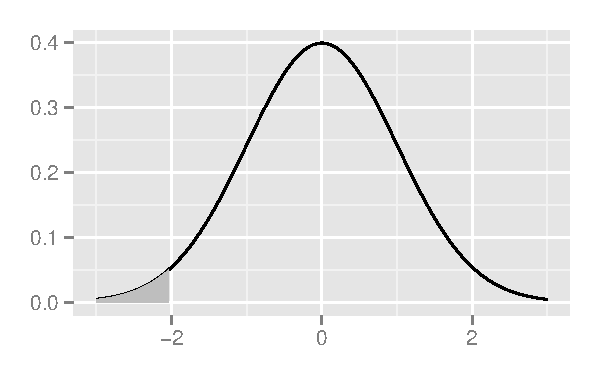
\includegraphics{figures/ex28a.pdf}
          \caption{Exercise 28 (a)}
        \end{figure}

        \begin{figure}[H]
          \centering
          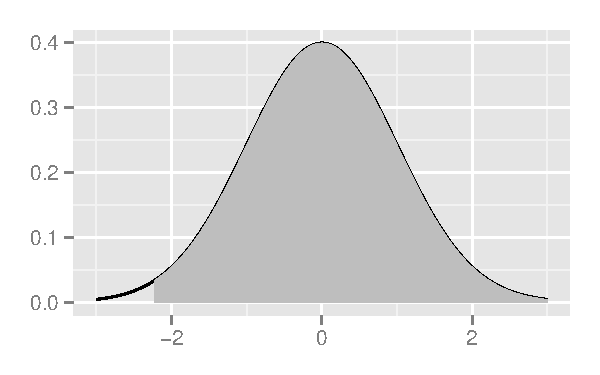
\includegraphics{figures/ex28b.pdf}
          \caption{Exercise 28 (b)}
        \end{figure}

        \begin{figure}[H]
          \centering
          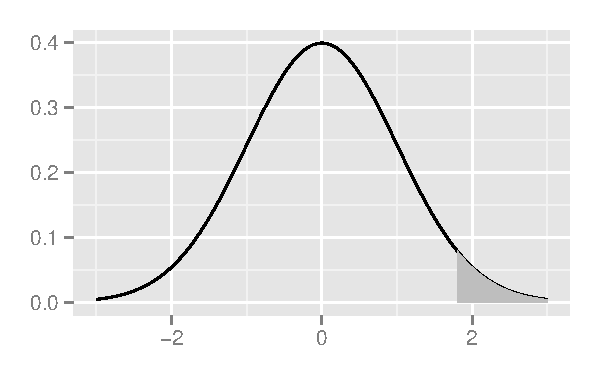
\includegraphics{figures/ex28c.pdf}
          \caption{Exercise 28 (c)}
        \end{figure}

        \begin{figure}[H]
          \centering
          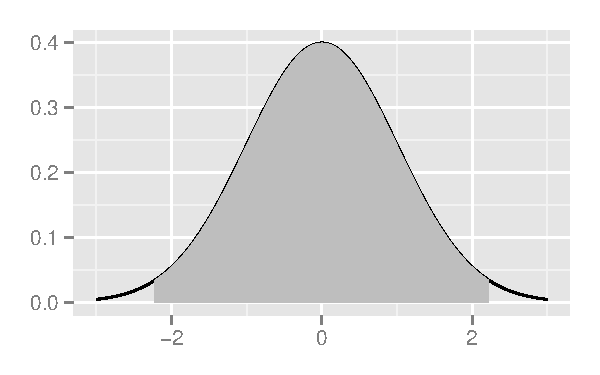
\includegraphics{figures/ex28d.pdf}
          \caption{Exercise 28 (d)}
        \end{figure}

      \item[29]
        \begin{parts}
          \part{} $z = 0.84$
          \part{} $z = 0.39$ 
        \end{parts}

      \item[30]
        Standardize:
        \[
          z = \frac{5 - 7.11}{0.74} = -2.8513
        \]

        Use table A:\@
        \[
          proportion = \boxed{ 0.0022 } 
        \]

      \item[31]
        Standardize:
        \[
          z = \frac{5 - 5.4}{0.54} = -0.7407407
        \]

        Use table A:\@
        \[
          proportion = \boxed{ 0.2296 } 
        \]

      % \item[32]
      %   \begin{parts}
      %     \part{} 
      %       Standardize:
      %       \[
      %         z = \frac{130 - 104}{12.5} = 2.08
      %       \]

      %       Use table A to find the percentage with heart rates below 130: 
      %       \[
      %         p_{below} = 98.12 \%
      %       \]

      %       Subtract from 100\% to find the percentage with heart rates above
      %       130:
      %       \[
      %         p_{above} = \boxed{ 1.876 \% }
      %       \]

      %     \part{}
      %       For the non-runners, 130 is the mean, so 50\% of the non-runners
      %       are above 130.

      %   \end{parts}

      \item[33]
        Standardize:
        \begin{align*}
          z_{\min} & = \frac{0.8720 - 0.8750}{0.0012} = -2.5 \\
          z_{\max} & = \frac{0.8780 - 0.8750}{0.0012} = 2.5 \\
        \end{align*}

        Use table A to find the proportions below the min/max
        \begin{align*}
          p_{\min} & = 0.006210 \\
          p_{\max} & = 0.9938 \\
        \end{align*}

        Subtract to find the proportion that meet the specifications:
        \[
          p_{good} = 0.9938 - 0.00621 = \boxed{ 0.9876 }
        \]

      \item[34]
        \begin{parts}
          
          \part{}
            Standardize:
            \begin{align*}
              z_{\min} &= \frac{11.2 - 11.5}{0.2} = -1.5 \\
              z_{\max} &= \frac{12.2 - 11.5}{0.2} = 3.5 \\
            \end{align*}

            Use table A to find the proportions below the min/max
            \begin{align*}
              p_{\min} & = 0.0668 \\
              p_{\max} & = 0.9998 \\
            \end{align*}

            Subtract to find the proportion that meet the specifications:
            \[
              p_{good} = 0.9998 - 0.0668 = \boxed{ 0.9330 }
            \]

            \part{}
              Standardize:
              \begin{align*}
                z_{\min} &= \frac{11.2 - 11.7}{0.2} = -2.5 \\
                z_{\max} &= \frac{12.2 - 11.7}{0.2} = 2.5 \\
              \end{align*}

              Use table A to find the proportions below the min/max
              \begin{align*}
                p_{\min} & = 0.0062 \\
                p_{\max} & = 0.9938 \\
              \end{align*}

              Subtract to find the proportion that meet the specifications:
              \[
                p_{good} = 0.9938 - 0.0062 = \boxed{ 0.9876 }
              \]

        \end{parts}

      \item[35]
        Standardize:
        \[
          z = \frac{25 - 18.7}{4.3} = 1.4651 \\
        \]

        Use table A:\@
        \[
          p = \boxed{ 92.86 \% } \\
        \]

      \item[36]
        Use table A to find how many standard deviations above the mean 90\% is: 
        \[
          z = \unit[1.2816]{sd}
        \]

        Convert to MPG
        \[
          x = 18.7 + 1.2816 \cdot 4.3 = \unit[24.21]{MPG}
        \]

      \item[37]
        Use table A:\@
        \begin{align*}
          z_{.25} &= \unit[-0.6745]{sd} \\
          z_{.75} &= \unit[0.6745]{sd} \\
        \end{align*}

        Convert to MPG
        \begin{align*}
          x_{0.25} &= 18.7 - 0.6745 \cdot 4.3 = \boxed{ \unit[15.8]{MPG} } \\
          x_{0.75} &= 18.7 + 0.6745 \cdot 4.3 = \boxed{ \unit[21.6]{MPG} } \\
        \end{align*}

      \item[43]
        \begin{parts}
          \part{}
            Standardize:
            \[
              z = \frac{750 - 533}{116} = 1.8707 \\
            \]

            Use table A:\@
            \[
              x = \boxed{ 3.07 \% }
            \]

          \part{}
            Standardize:
            \[
              z = \frac{750 - 499}{110} = 2.2818 \\
            \]

            Use table A:\@
            \[
              x = \boxed{ 1.13 \% }
            \]

        \end{parts}

      \item[44]
        Use table A:i\@
        \begin{align*}
          z_{0.1} &= -1.28 \\
          z_{0.9} &= 1.28 \\
        \end{align*}

        Find the mean and standard deviation:
        \begin{align*}
          \mu - 1.28 \sigma &= 25 \\
          \mu + 1.28 \sigma &= 475 \\
          \\
          2 \mu & = 500 \\
          \mu   & = 250 \\
          \\
          250 + 1.28 \sigma & = 475 \\
          \sigma            & = 175.78 \\
        \end{align*}

        The distribution is \fbox{ $N(250, 176)$ }

      \item[46]
        \begin{figure}[H]
          \centering
          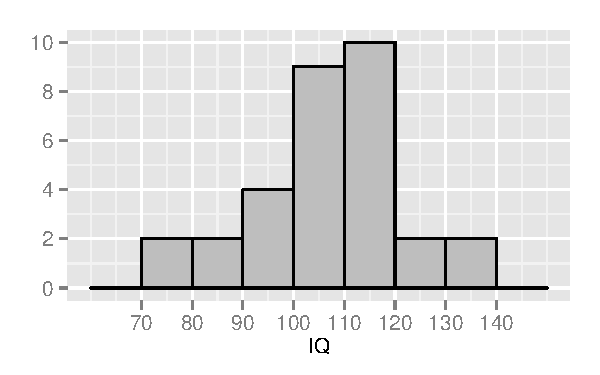
\includegraphics{figures/ex46.pdf}
          \caption{Exercise 46}
        \end{figure}

        \begin{align*}
          \mu    & = 105.84 \\
          \sigma & = 14.27
        \end{align*}

        \begin{tabular}[H]{llrr}
          \toprule
          $\sigma$ & Range             & Expected & Actual \\
          \midrule
          1         & $(120.11, 91.57)$ & 21       & 23 \\
          2         & $(77.30, 104.38)$ & 29       & 29 \\
          \bottomrule
        \end{tabular}

        The actual and expected are pretty close.  There are a few more students than you
        would expect within one standard deviation of the mean.  

      \pagebreak

      \item[48]
        \begin{parts}
          \part{} 
            \begin{itemize*}
              \item The mean and median are nearly identical (5.43 vs. 5.44).

              \item The first and third quartiles are about the same distance from the
                mean (0.39 vs. 0.35)

              \item The min is closer to the mean than the max (1.11 vs. 1.37) 
            \end{itemize*}

            Since the max is a bit larger than you would expect, the data seems asymmetric
            and skewed to the right.  However, since the mean and max are nearly
            identical, there can't be too many observations at the high end of the range
            since if there were, the mean would be bigger than the median.

        \part{}
          Standardize:
          \begin{align*}
            z_1 & = \frac{5.05 - 5.43}{0.54} = -0.7037 \\
            z_2 & = \frac{5.79 - 5.43}{0.54} = 0.6668 \\
          \end{align*}

          Use table A:\@
          \begin{align*}
            p_1 & = 24.08 \% \\
            p_2 & = 74.25 \% \\
          \end{align*}

          These distributions are almost exactly what you would expect for a
          normal distribution.  There are probably only one or two big samples
          at the high end of the range.  This would explain the high maximum
          value with everything else being what you would expect from a normal
          distribution.

        \end{parts}


    \end{description}

  \else
    \vspace{9 cm}
    \begin{quote}
      \begin{em}
        They see a race of law-makers legislating without knowing what their
        laws are about; today voting a law on the sanitation of towns, without
        the faintest notion of hygiene, tomorrow making regulations for the
        armament of troops, without so much as understanding a gun; making laws
        about teaching and education without ever having given a lesson of any
        sort, or even an honest education to their own children; legislating at
        random in all directions, but never forgetting the penalties to be meted
        out to ragamufffins, the prison and the galleys, which are to be the
        portion of men a thousand times less immoral than these legislators
        themselves
      \end{em}
    \end{quote}
    \hspace{1 cm} --Peter Kropotkin
  \fi

\end{document}

